The sensitivity of the asymmetry measurement can be diluted due to detector and reconstruction effects, which can be parametrized through a dilution factor (\dilution).
The \Acpprime and \Acp values are related through \dilution, applied as a multiplicative correction $\Acpprime = \dilution \Acp$~\cite{CPVtop:13TeVRef}.
The dilution factor can be defined as
\begin{linenomath}\begin{equation}
    \dilution = \epsc - \epsw,
\end{equation}\end{linenomath}
where \epsc is the fraction of events where the measured CP observable has the correct sign, and \epsw is the fraction with the wrong sign.
Events are classified into the correct-sign (wrong-sign) type when the sign of the CP observable at the reconstruction level agrees with (differs from) that at the \POWHEG generator level.

The value of \dilution depends on the final-state objects used to form each CP observable.
In contrast to \Otwelve and \Ofourteen, it is necessary for \Othree and \Osix to distinguish the charges of the \PQb quarks by using the sign of the lepton charge, and therefore they tend to have a lower fraction of correct-sign events and smaller values of \dilution.
The value of \dilution can also be affected by possible contributions of BSM processes, because the CP observables are reconstructed using kinematic features of the final-state objects.
The model-dependency in the dilution factor of each observable is studied using SM simulated \ttbar samples and CEDM model simulated \ttbar samples.
Figure~\ref{fig:DF_CEDM_SM} shows that the differences between different models are negligible and consistent with unity within one standard deviation in the low \dtG region.
The values of \dilution determined from the SM simulations are given in Table~\ref{tab:dilution_factor}, along with their systematic uncertainties described in Section~\ref{sec:uncertainty}.

\begin{figure}
    \centering
    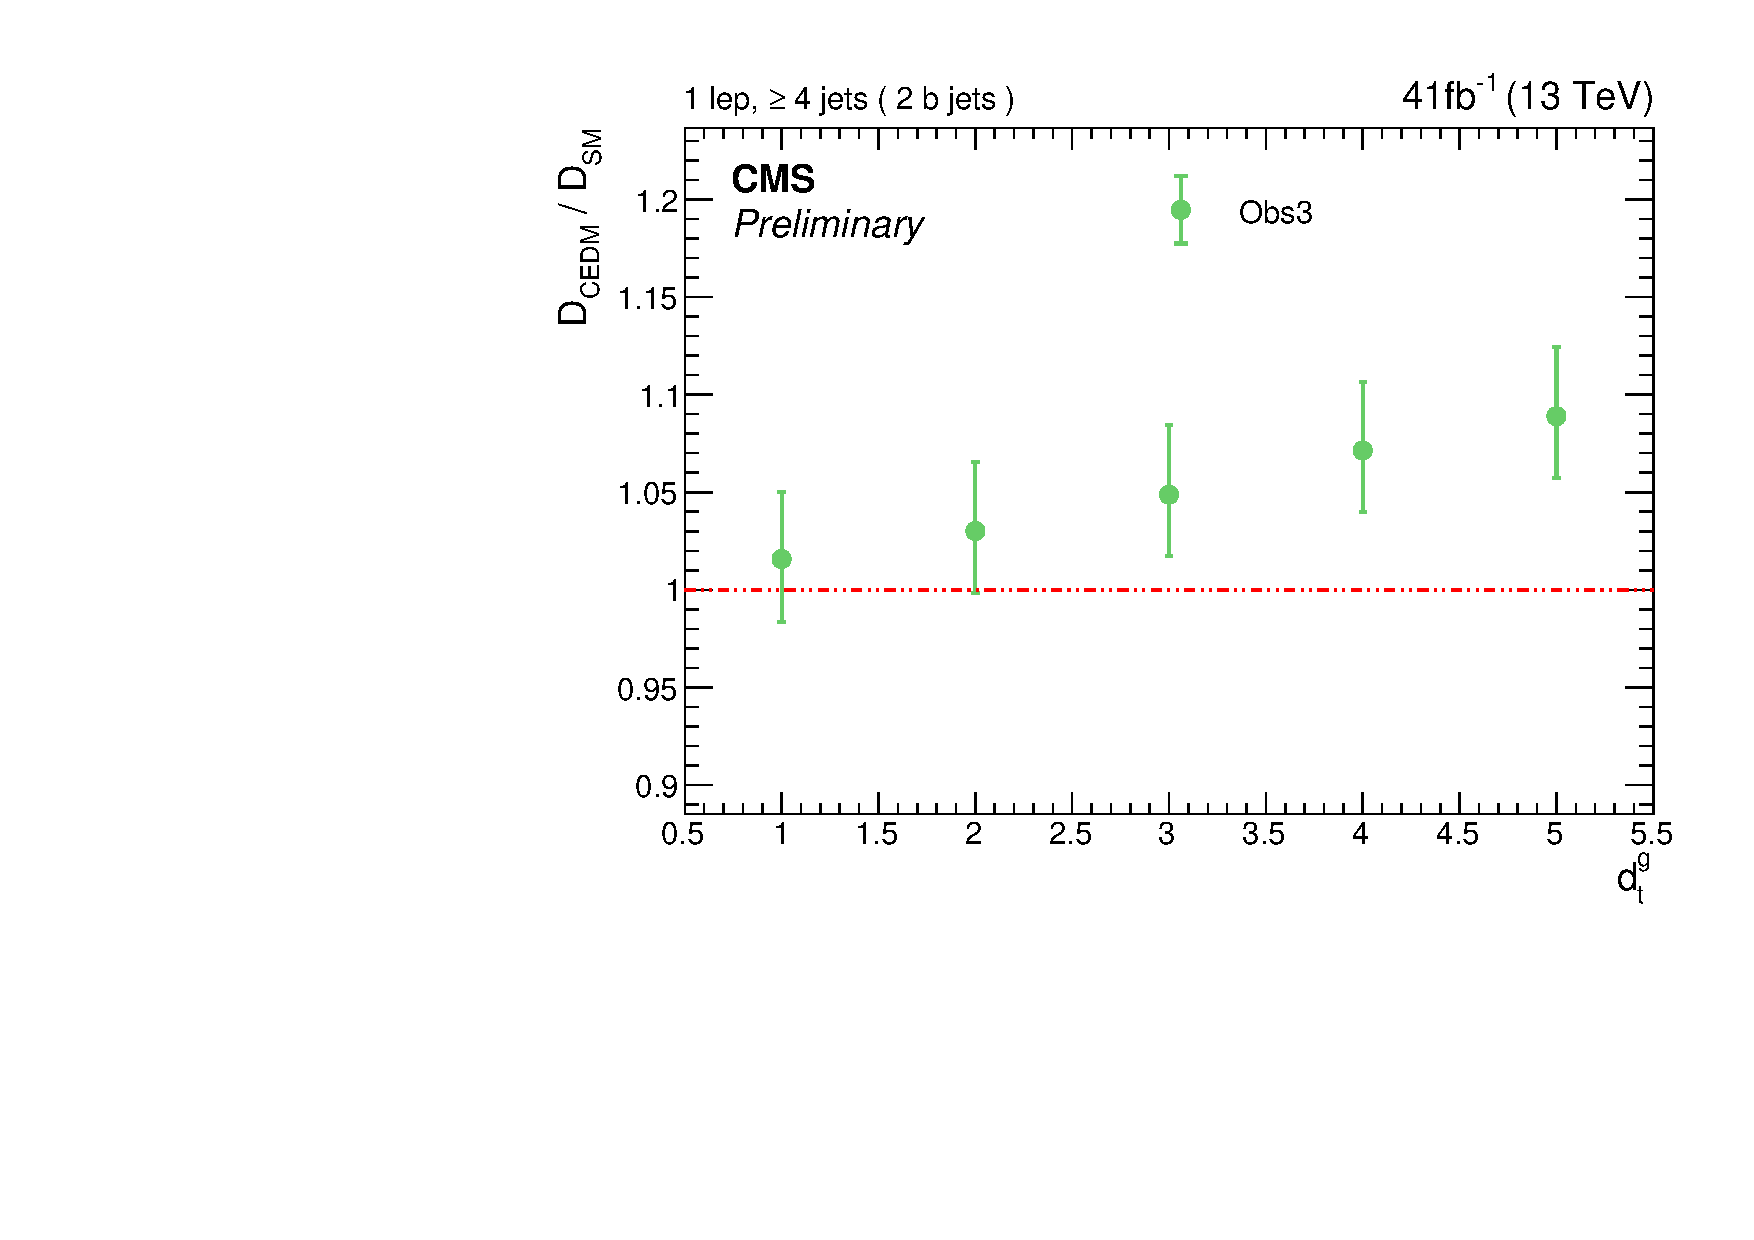
\includegraphics[width=0.45\textwidth]{figure/Ratio_17_co_DF_Obs3_chi2_20_opt_150.pdf}
    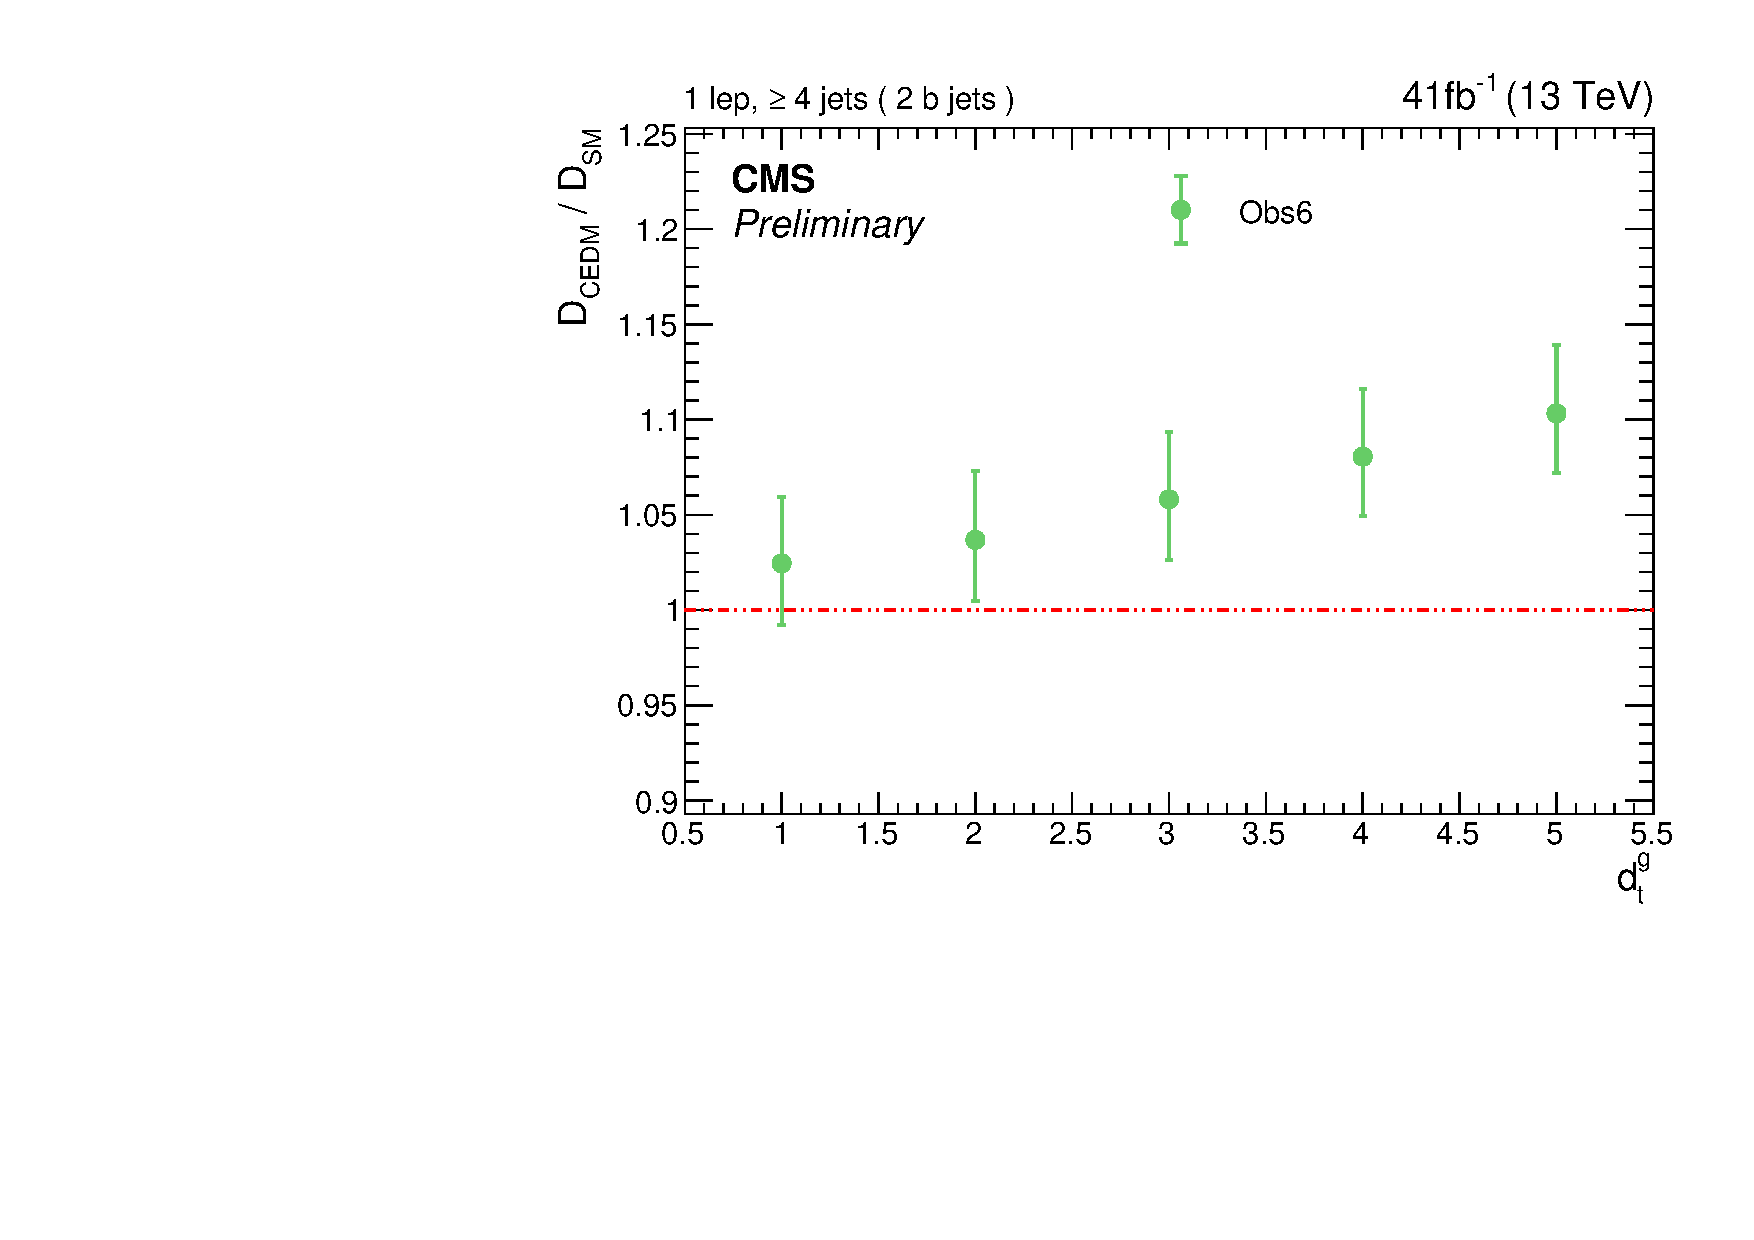
\includegraphics[width=0.45\textwidth]{figure/Ratio_17_co_DF_Obs6_chi2_20_opt_150.pdf}
    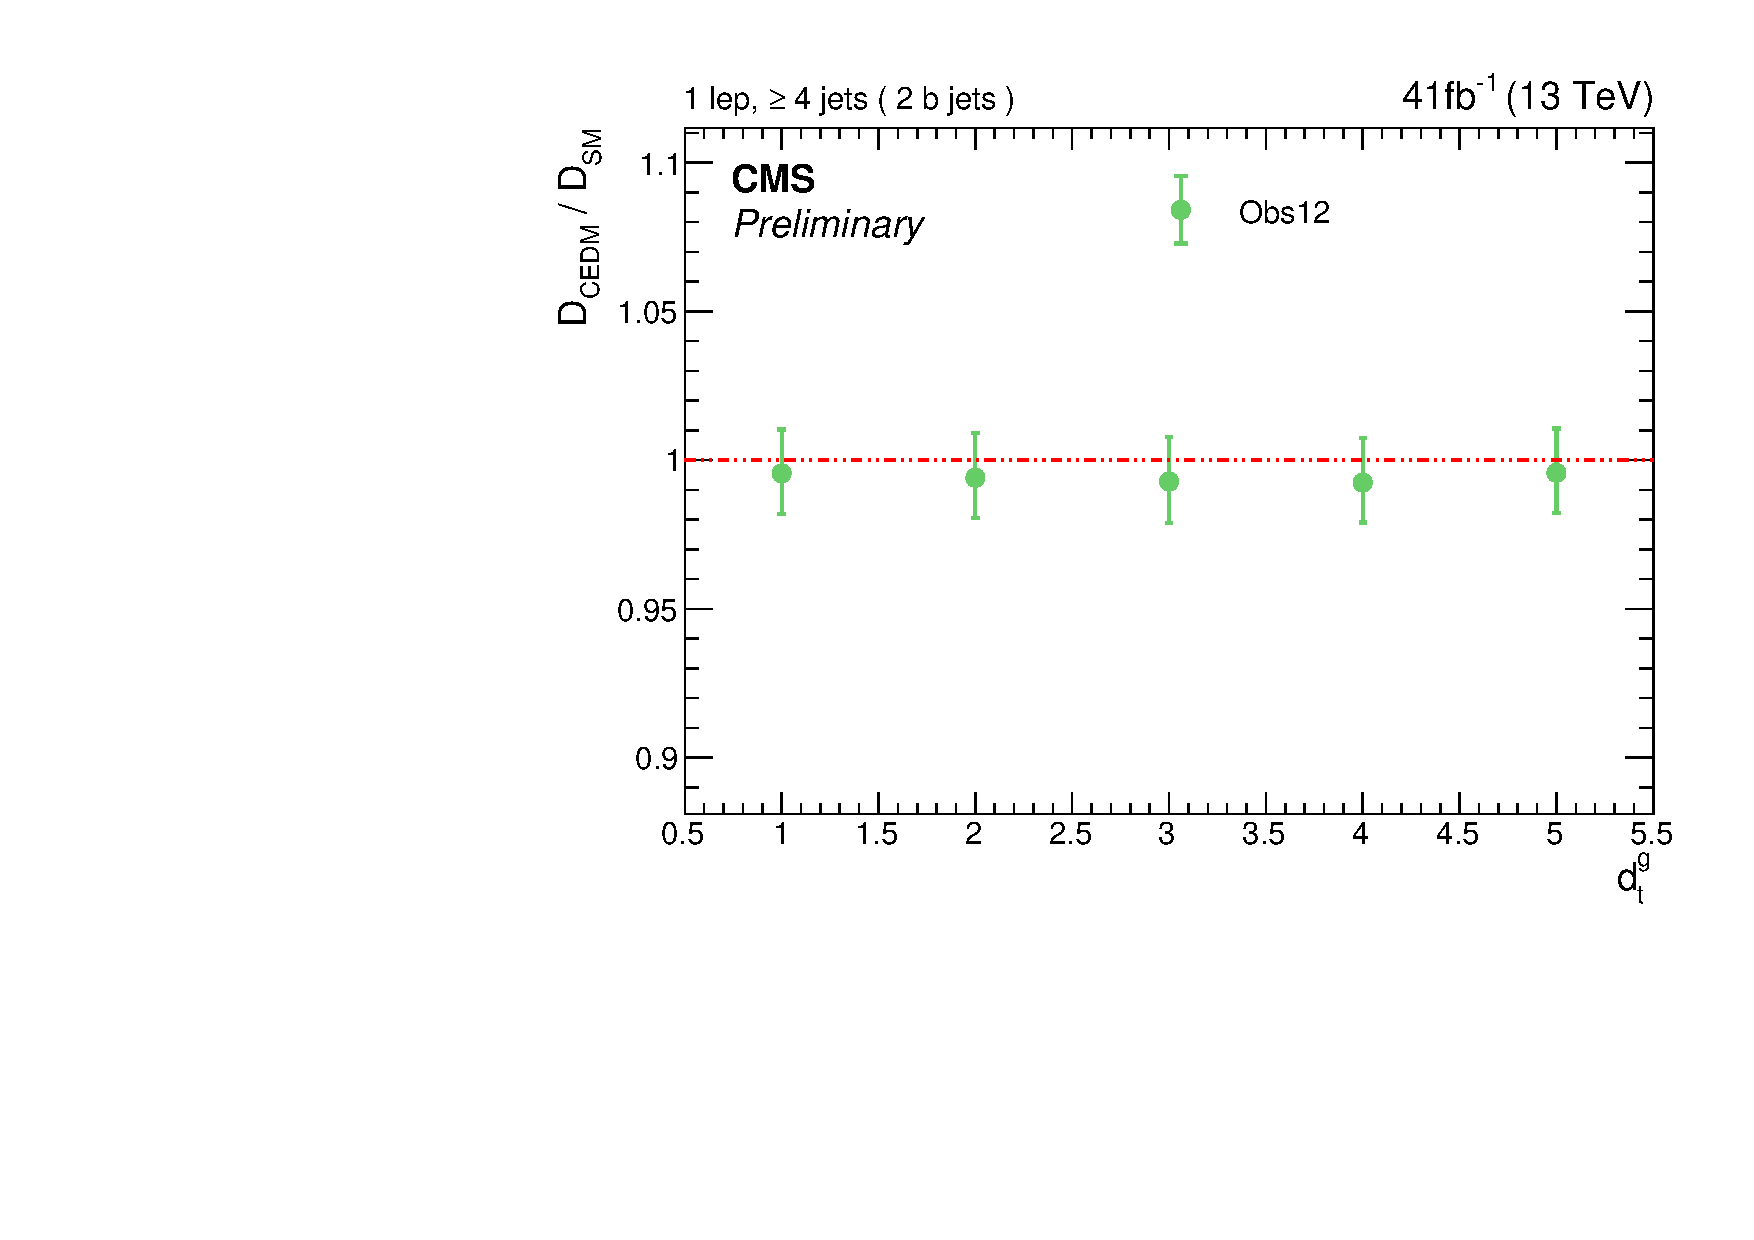
\includegraphics[width=0.45\textwidth]{figure/Ratio_17_co_DF_Obs12_chi2_20_opt_150.pdf}
    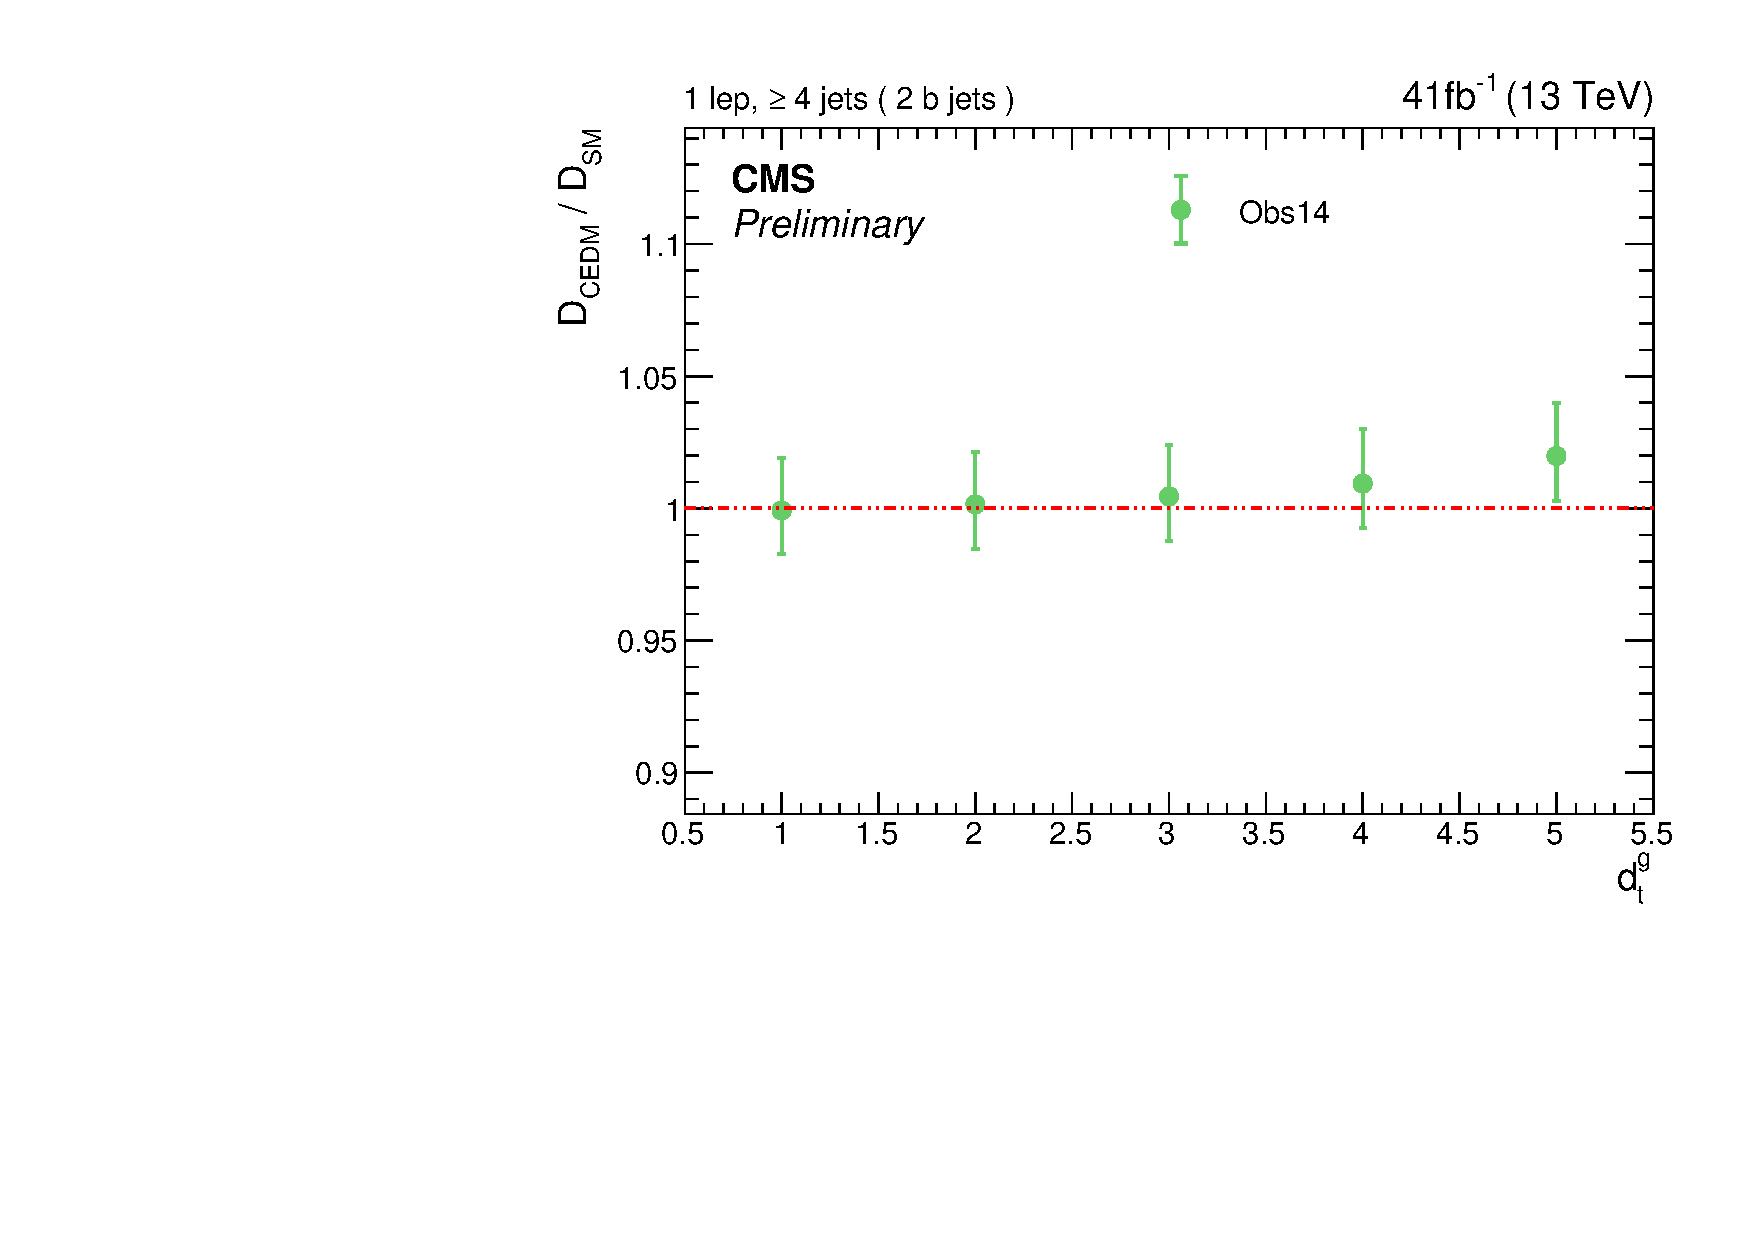
\includegraphics[width=0.45\textwidth]{figure/Ratio_17_co_DF_Obs14_chi2_20_opt_150.pdf}
    \caption[Model dependency for the dilution factor for each observable.]
    {
        Model dependency for the dilution factor for each observable. 
        The points show the ratio between the value obtained by re-weigthing events according to different CEDM models with the baseline results obtained in the SM simulation.
        It should be noticed that, although all the points are correlated, the deviations from unity are much smaller than the statistical error represented by the error bars in the low \dtG region.
    }
    \label{fig:DF_CEDM_SM}
\end{figure}

\begin{table}[!h]
    \caption[The dilution factor \dilution for each CP observable.]
    {
        The dilution factor \dilution determined from simulation and its systematic uncertainty for each CP observable.
        The statistical uncertainty is negligible compared to the systematic uncertainty.
    }
    \label{tab:dilution_factor}
    \centering\renewcommand\arraystretch{1.4}
    \begin{tabular}{cc}
        CP observable & Dilution factor \dilution \\
        \hline
        \Othree  & $0.46\,^{+0.01}_{-0.02}$\\
        \Osix  & $0.44\,^{+0.01}_{-0.02}$\\
        \Otwelve & $0.74\,^{+0.01}_{-0.02}$\\
        \Ofourteen & $0.60\,^{+0.01}_{-0.01}$\\
    \end{tabular}
\end{table}

In order to better understand the measured \dilution values, the lepton+jets and dilepton+jets events in the simulated \ttbar samples are reweighted at the generator level to produce various pseudo-asymmetry values.
The SM simulated \ttbar events can be reweighted as 

\begin{align}
    w^{+}_i &= 1 + A_{CP}(O_i) \\
    w^{-}_i &= 1 - A_{CP}(O_i) 
\end{align}

where \Acp$(O_i)$ is the input artificial \Acp value for each observable, $w^{+(-)}_i$ is a weight for events with positive (negative) value of $O_i$ at generator level.
For example, if we want to have $+5\%$ \Acp value in \Othree, the event weight for $w^{+}_{3}$ will be $1.05$ and $w^{-}_{3}$ will be $0.95$. 
As shown in Fig.~\ref{fig:check_dilution_factor}, the CP-violating asymmetries \Acp (diamond points) are then obtained by dividing the effective asymmetries \Acpprime (circular points) by the corresponding dilution factor determined from simulation.
Fitting the \Acpprime and \Acp values to linear functions of the generator-level pseudo-asymmetry values results in the red-dotted and blue-solid lines shown in Fig.~\ref{fig:check_dilution_factor}, respectively.
All the fits have good \chisq values, and the slopes and $y$ intercepts of the fitted lines to \Acp are consistent with 1.0 and 0.0, respectively.

\begin{figure}[h!]
    \centering
    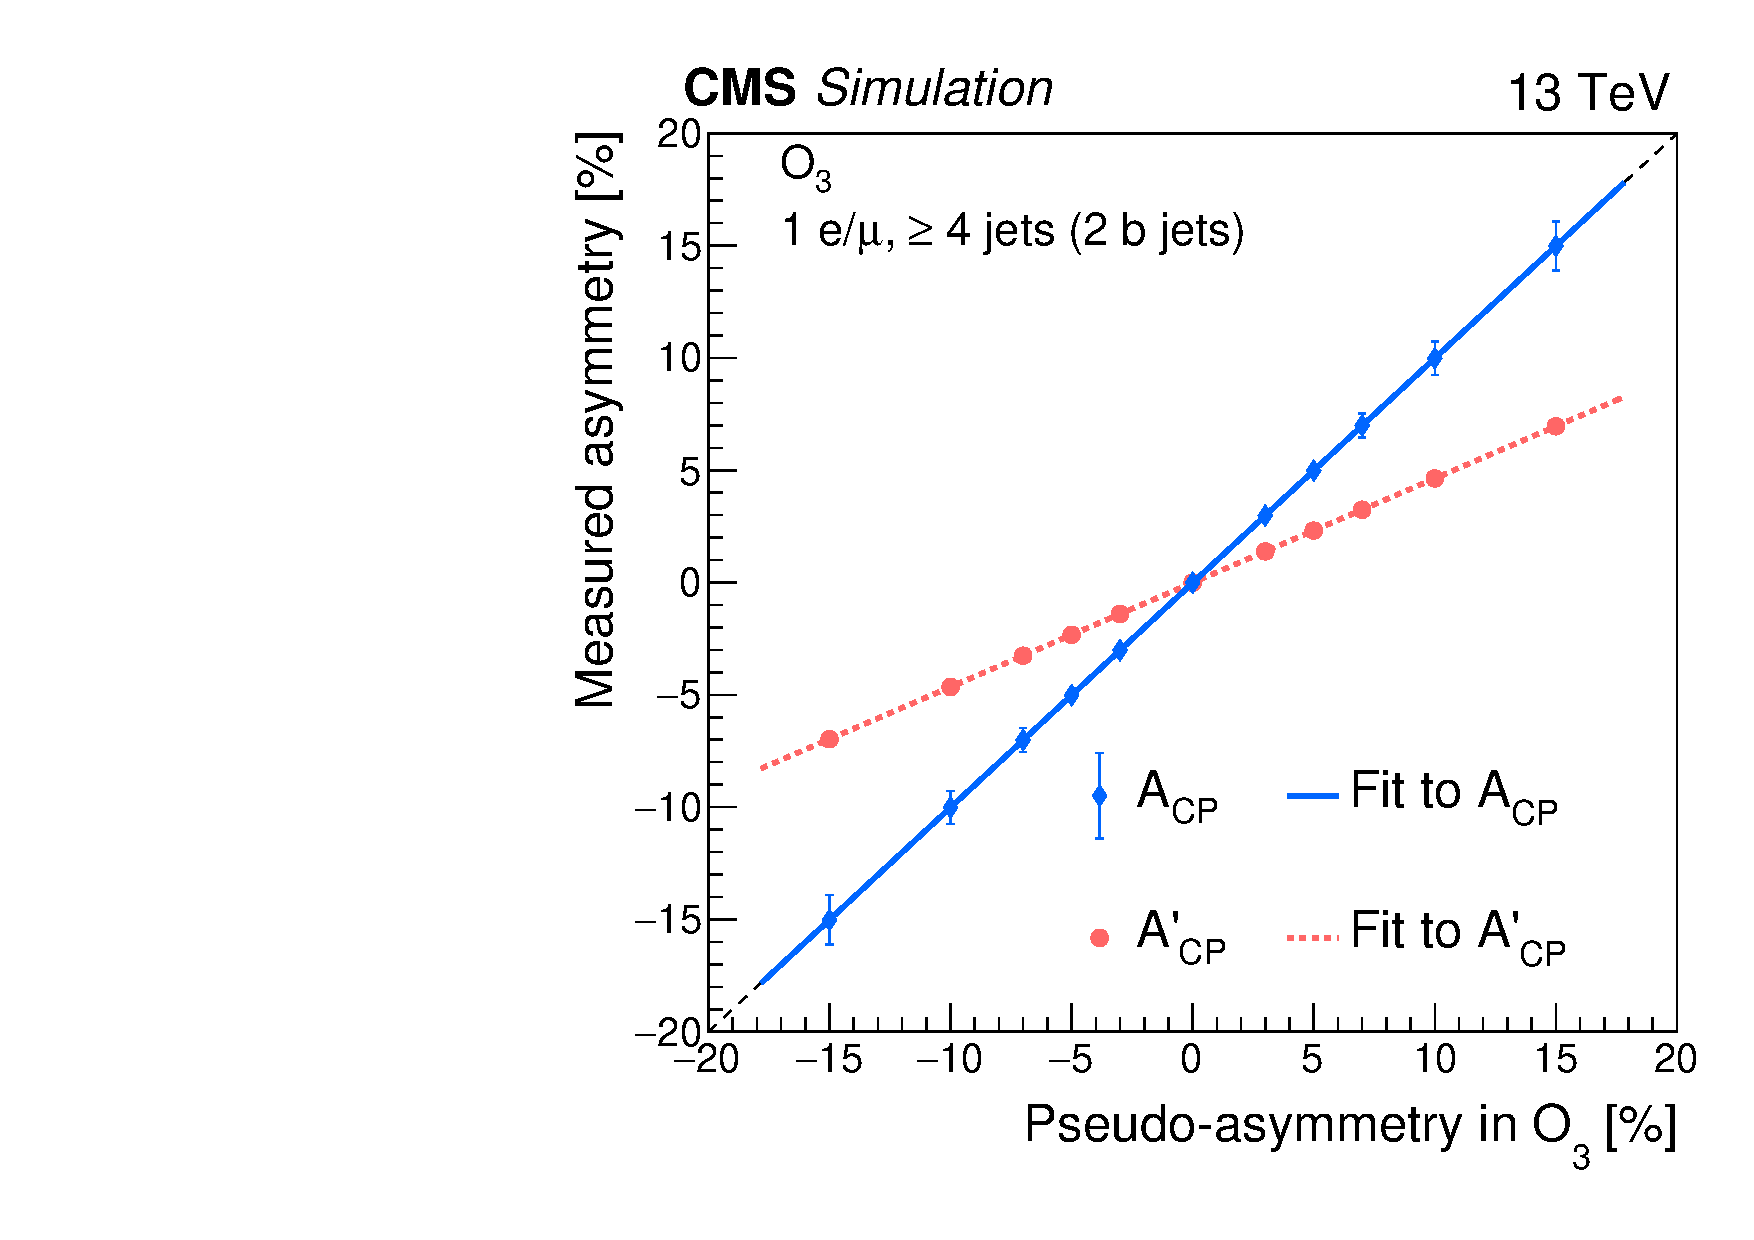
\includegraphics[width=0.45\textwidth]{figure/Figure_005-a.pdf}
    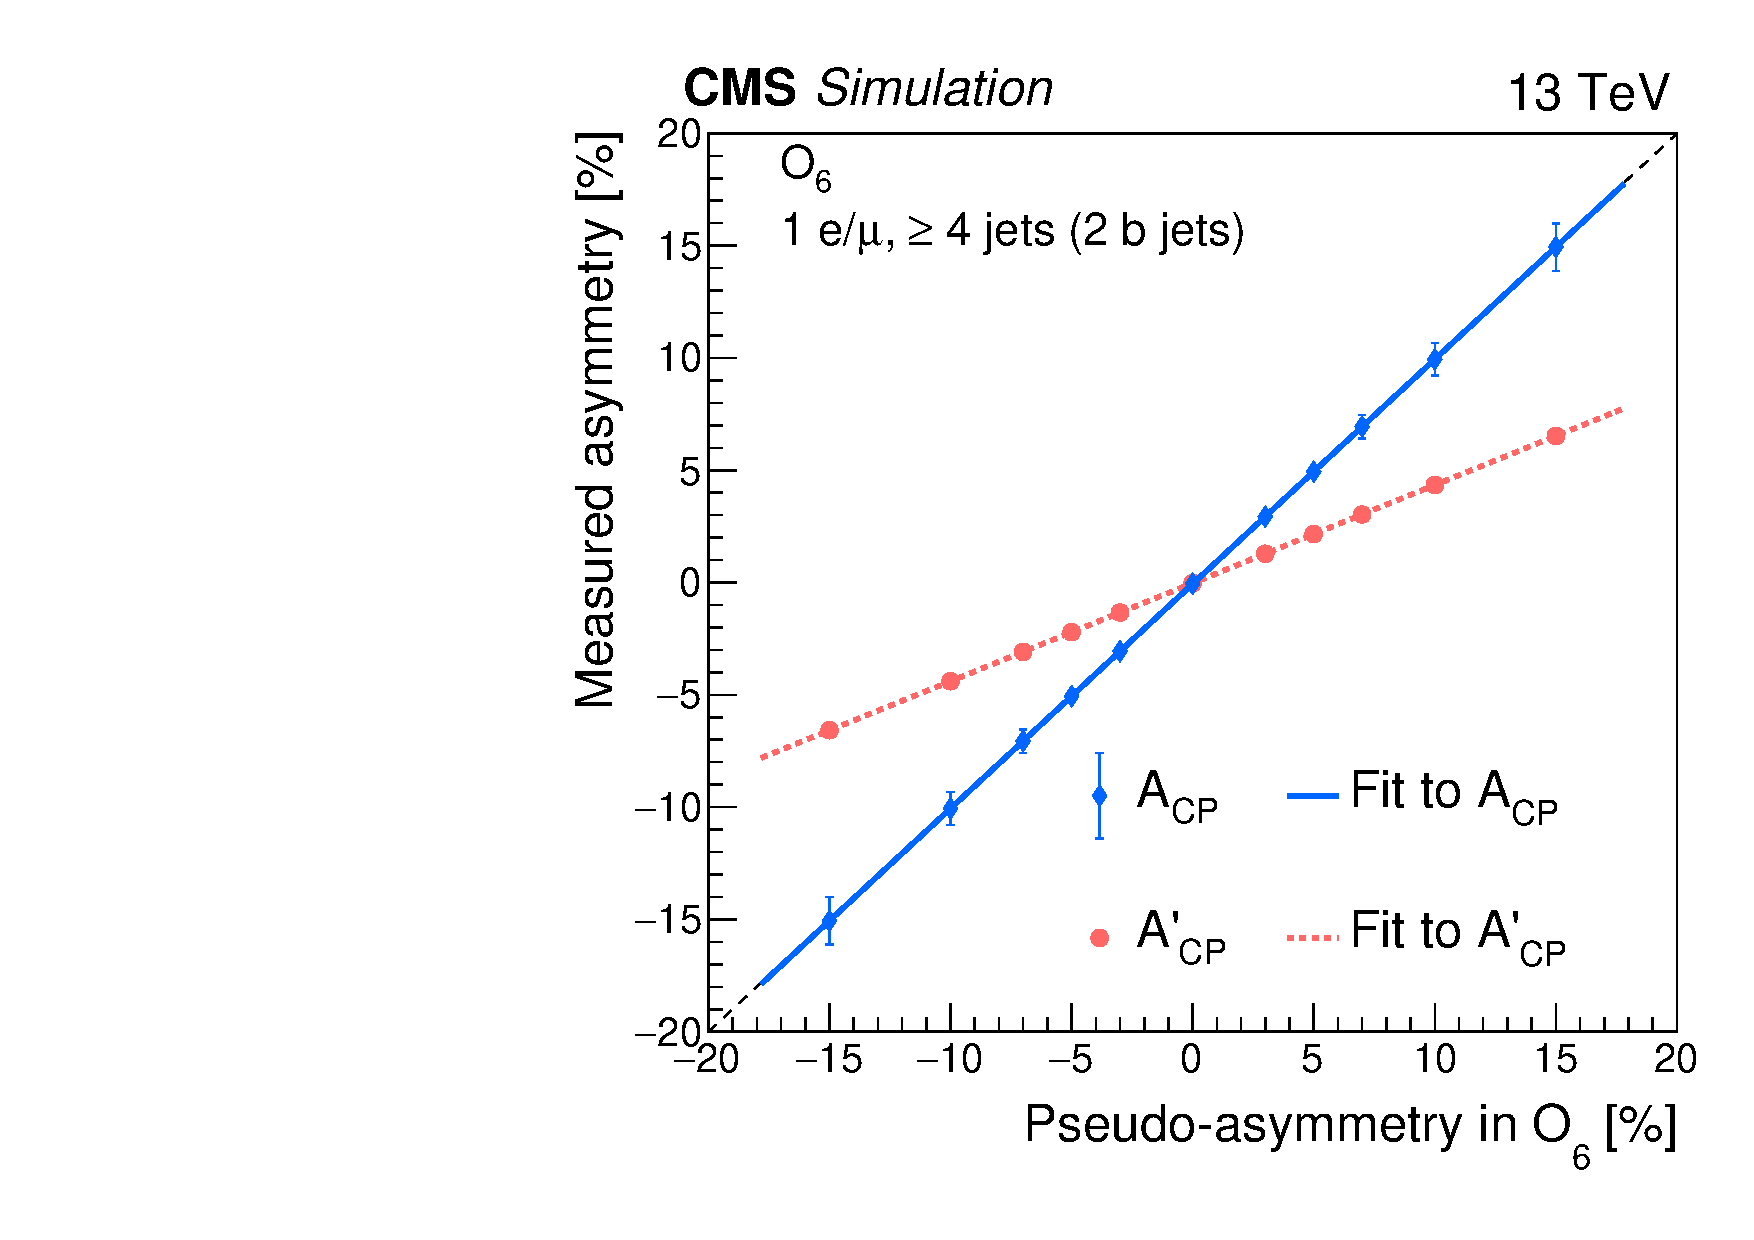
\includegraphics[width=0.45\textwidth]{figure/Figure_005-b.pdf}
    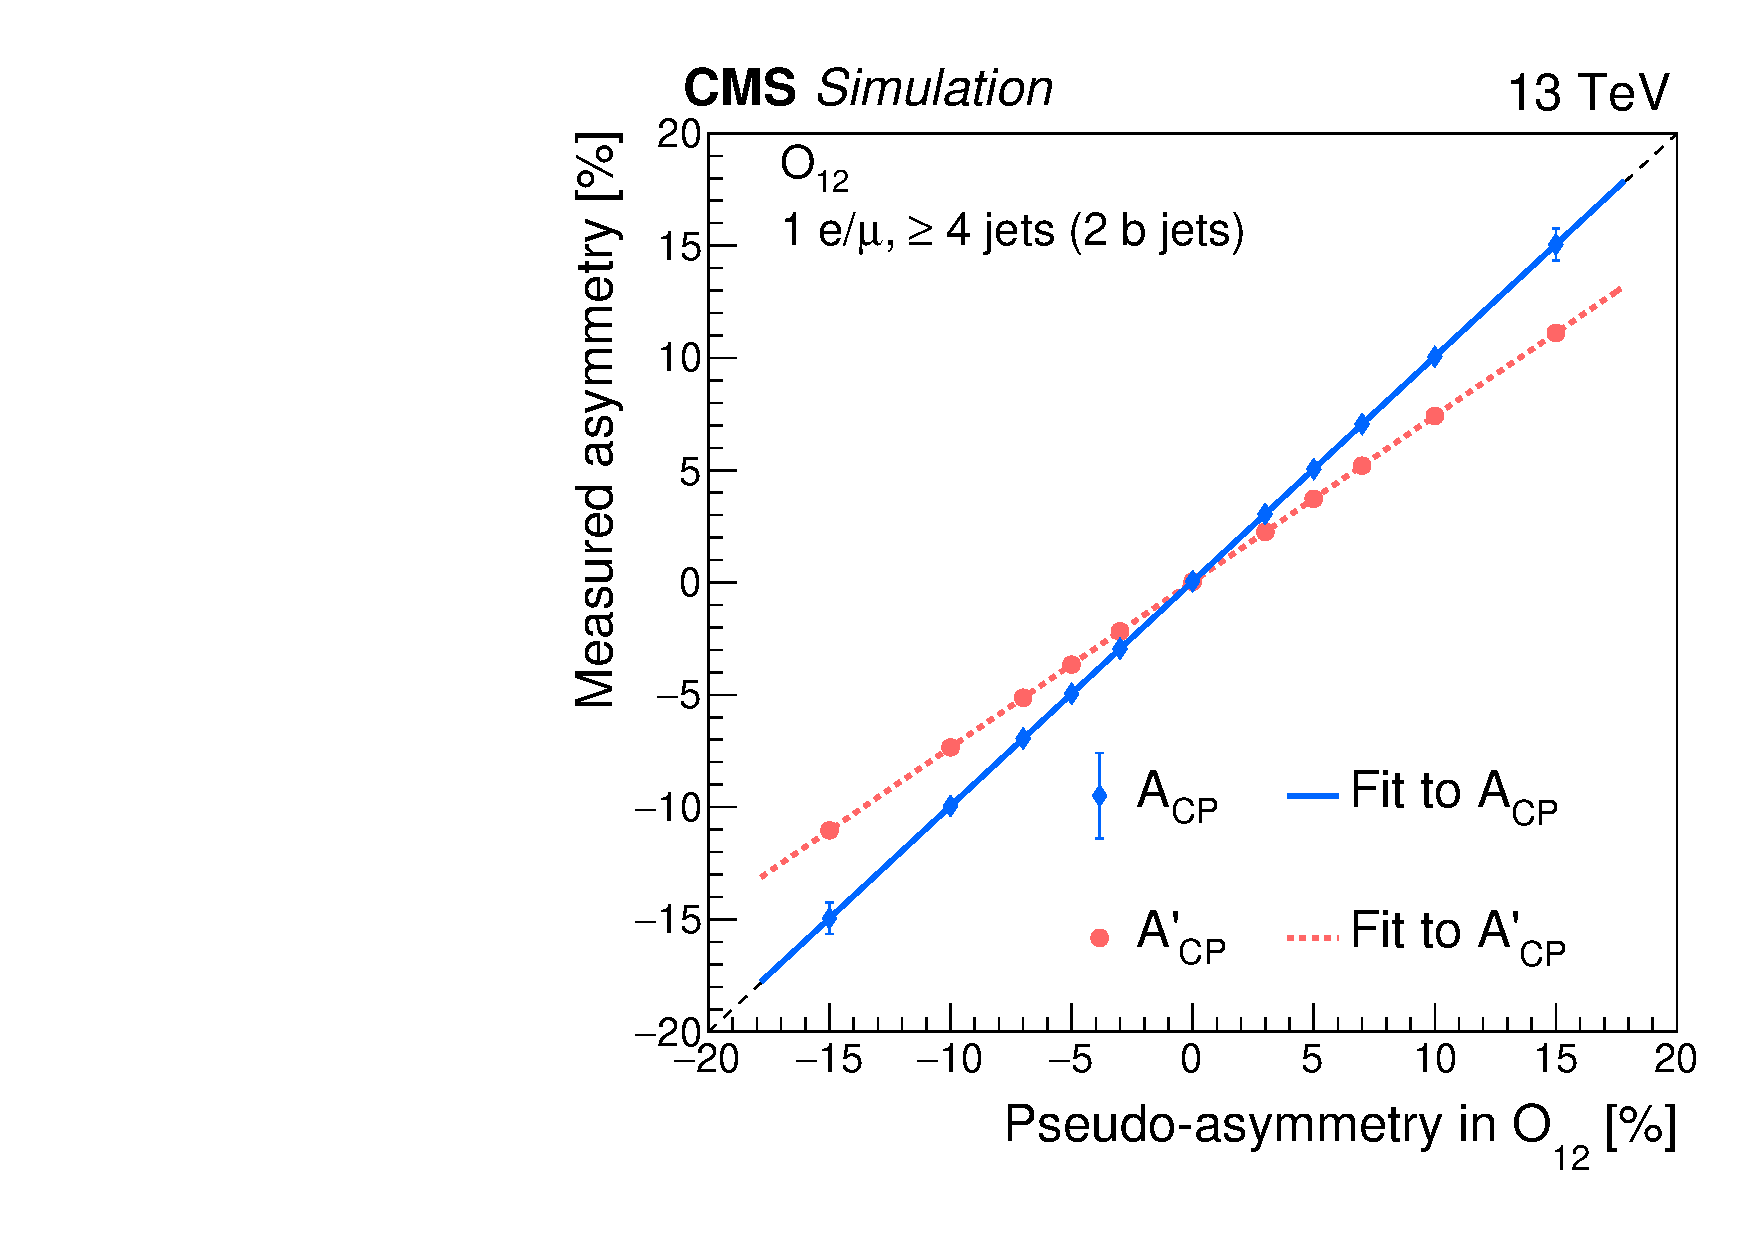
\includegraphics[width=0.45\textwidth]{figure/Figure_005-c.pdf}
    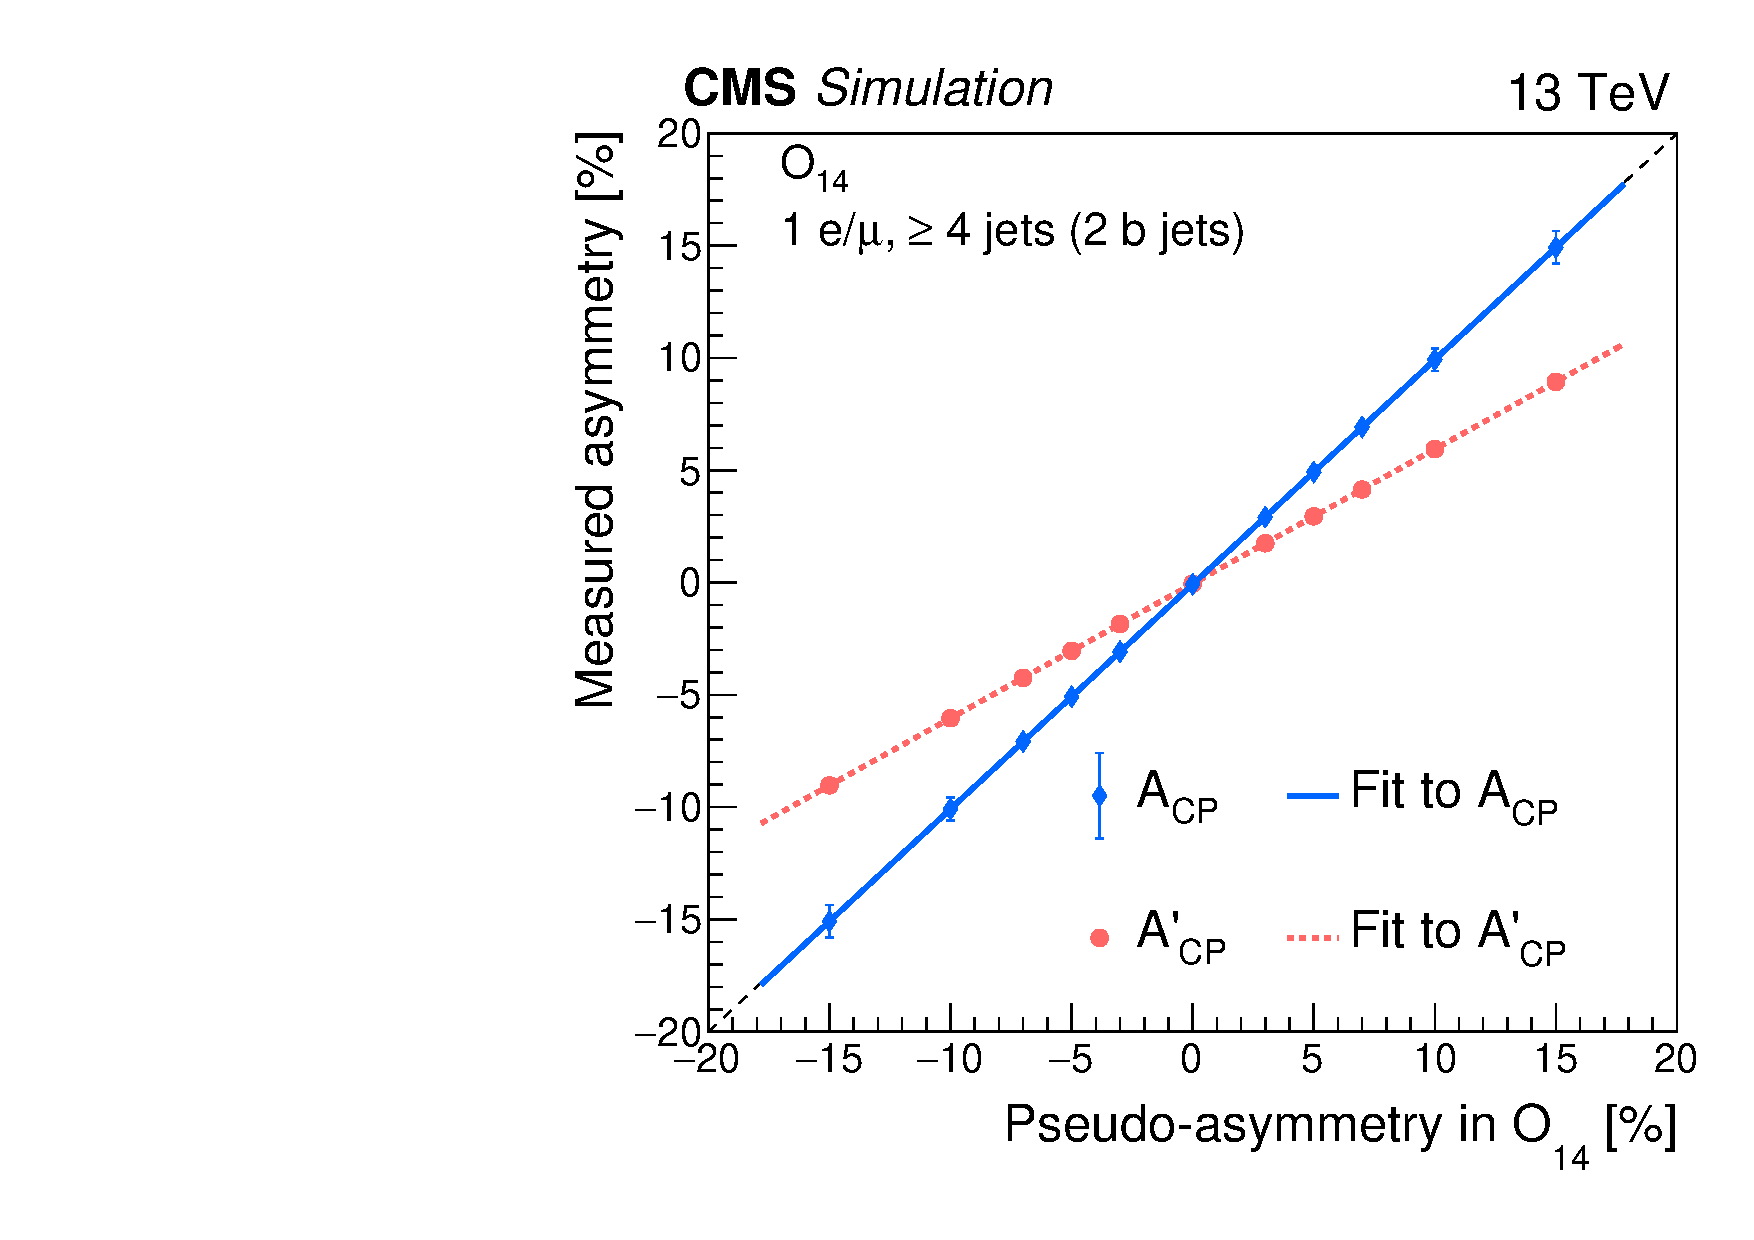
\includegraphics[width=0.45\textwidth]{figure/Figure_005-d.pdf}
    \caption[The measured CP-violating asymmetries as a function of the pseudo-asymmetry.]
    {
        The measured CP-violating asymmetries in simulation as a function of the generator-level pseudo-asymmetry for the CP observables \Othree (upper left), \Osix (upper right), \Otwelve (lower left), and \Ofourteen (lower right).
        The red circles and blue diamonds give the \Acpprime and \Acp values, respectively, with the red-dotted and blue-solid lines showing the results of linear fits to those corresponding values.
        The \Acp value is obtained by dividing the \Acpprime value by the dilution factor determined from simulation for that CP observable.
        The statistical uncertainties in the \Acpprime values are smaller than the markers.
    }
    \label{fig:check_dilution_factor}
\end{figure}
